\documentclass{tietreport}
\usepackage{booktabs,tabularx,array,float}
\usepackage[T1]{fontenc}
\usepackage{lmodern}
\usepackage{emptypage}
\hypersetup{hidelinks,pdftitle={Carelane: Project Progress Report},pdfauthor={Pranshu Sharma; Shashwat Mishra; Mayank Kalra}}
\setlength{\headheight}{15pt}
\setlength{\emergencystretch}{2em}
\renewcommand{\arraystretch}{1.2}
\raggedbottom
\newcolumntype{Y}{>{\raggedright\arraybackslash}X}
\graphicspath{{figures/}}

% Complete the marked administrative fields before submission.
\TitlePageHeader{UCS503P -- Software Engineering Project Report}
\ProjectTitle{Carelane}
\ProjectSubTitle{AI-Assisted Healthcare Guidance,\\Appointment Booking and Queue Estimation\\[0.15cm]Project Progress Report}
\author{Pranshu Sharma \quad {\small [Roll number]}\\[0.12cm]
Shashwat Mishra \quad {\small [Roll number]}\\[0.12cm]
Mayank Kalra \quad {\small [Roll number]}}
\TitlePageSubText{Group: [Group number]\\B.E. Third Year, Computer Engineering (COE)}
\AdvisorName{[Faculty / Guide name]}
\TitlePageFooterText{{\large Mid-Semester Evaluation}\\[0.2cm]
\textbf{Computer Science and Engineering Department}\\[0.15cm]
Thapar Institute of Engineering and Technology, Patiala\\[0.15cm]
14 September 2026}

\begin{document}
\maketitle
\tableofcontents

\chapter{Introduction}
\section{Background and Context}
Carelane is an educational software engineering project that combines text-based specialty guidance with an appointment and queue-management prototype. The intended experience is a single patient-facing application: enter a symptom description, explore a department, choose a doctor and time, and follow the progress of a visit. A companion browser interface makes the workflow accessible on a laptop and supports demonstration and evaluation.

The work completed so far has two distinct parts. The machine-learning part prepares a public symptom-description dataset, trains and evaluates classifiers, and develops a waiting-time regressor on simulated queue records. The software part connects a saved specialty model to a patient application, stores fictional appointments, and demonstrates queue movement. These components are integrated locally; no hospital partnership or clinical deployment has been completed.

This report documents the available implementation and saved evidence as of 14 September 2026. Model results refer to the latest saved runs from 6--7 September, and application verification refers to the recorded 9 September test run. No models were retrained merely to prepare this report. A subsequent local-care directory and interface redesign have been started but are not part of the validated application release.

\subsection{Problem Statement}
The project addresses a software workflow problem: a user may need help exploring an appropriate care department, keeping track of a booking, and understanding the progression of a visit. A directory alone does not demonstrate symptom interpretation, while a classifier alone does not provide an appointment workflow. Similarly, a waiting-time number without its assumptions can create an unjustified impression of precision.

The engineering challenge is therefore to connect these functions while preserving their boundaries. Experimental classifier outputs must remain suggestions for professional review. Simulated appointments must not be represented as real reservations, and queue estimates learned from a simulator must not be described as measured hospital performance. The two supplied project proposals also envision hospital discovery, staff and administration workspaces, secure records and real-time integrations. Those remain proposed capabilities rather than verified features of this iteration.

\section{Project Objectives}
The completed prototype was developed around the following objectives:
\begin{enumerate}
\item Establish a reproducible data preparation and training pipeline with saved models, metrics, configuration and provenance.
\item Compare a compact TF-IDF classifier with a fine-tuned transformer on the same specialty-label experiment.
\item Train a waiting-time estimator using chronological splits of simulated visits and compare it with a simple baseline.
\item Integrate the selected local specialty inference service into a responsive patient application.
\item Implement persistent demo bookings, cancellation, session-based ownership, and an explicit simulated queue.
\item Produce inspectable training logs, figures, screenshots and software tests for project documentation.
\end{enumerate}

\section{Scope and Current Status}
\begin{table}[H]\centering\small
\begin{tabularx}{\textwidth}{p{0.32\textwidth}Y}
\toprule Component & Status and evidence \\ \midrule
Data preparation & Implemented; dataset audit and split files saved. \\
Text models & Two Logistic Regression models and one fine-tuned DistilBERT model trained and evaluated. \\
Waiting-time model & CatBoost trained and evaluated on simulated FCFS visits. \\
Research dashboard & Local report page with metrics, training history and downloadable research assets. \\
Patient app & Tested browser prototype with guidance, fictional doctor search, bookings and queue controls. \\
Android support & JavaScript/Hermes bundle exported; no signed APK or physical-device verification recorded. \\
Real-care directory & Types, service route and draft components created; zero populated listings and no completed integration in the tested screen flow. \\
Clinical deployment & Not performed; no real patient validation, confirmed bookings or hospital integration. \\
\bottomrule
\end{tabularx}
\caption{Project status based on inspected files and saved validation records.}
\end{table}

\chapter{Methodology and Design}
\section{System Architecture}
\subsection{High-Level Design}
The application uses a client--service architecture. A React Native application built with Expo provides the patient interface. Its service client sends JSON requests to a local FastAPI process. The service calls the saved model for specialty suggestions and uses SQLite for demo sessions and appointments. Training and evaluation remain separate from the request-handling path.

\begin{figure}[H]\centering\small
\fbox{\parbox{0.88\textwidth}{\centering Expo / React Native patient app\\Symptom guide, doctor search, visits and queue screens}}
\par\vspace{0.15cm}$\updownarrow$\quad JSON over HTTP\par\vspace{0.15cm}
\fbox{\parbox{0.88\textwidth}{\centering FastAPI patient service\\Session ownership, validation and appointment transitions}}
\par\vspace{0.15cm}$\swarrow$\hspace{3cm}$\searrow$\par\vspace{0.15cm}
\begin{tabular}{cc}
\fbox{\parbox{0.39\textwidth}{\centering Local model artifacts\\Specialty baseline / queue model}} &
\fbox{\parbox{0.39\textwidth}{\centering SQLite database\\Sessions and demo appointments}}
\end{tabular}
\caption{Implemented patient-service architecture. The research dashboard reads saved evaluation artifacts separately.}
\end{figure}

A typical interaction starts with an anonymous demo session. The patient describes example symptoms, and the service returns three ranked specialty labels without presenting classifier scores as medical probabilities. The user can then browse fictional doctors, choose an available time and create a demo appointment. After check-in, queue state is refreshed every five seconds; a demo desk action explicitly advances fictional patients.

\subsection{Technical Stack}
\begin{table}[H]\centering\small
\begin{tabularx}{\textwidth}{p{0.25\textwidth}Y}
\toprule Layer & Tools and role \\ \midrule
Data processing & Python, pandas and NumPy for input preparation, audit and saved predictions. \\
Text baselines & scikit-learn TF-IDF, FeatureUnion, Logistic Regression; joblib persistence. \\
Transformer & Hugging Face Transformers and tokenizer; PyTorch, AdamW and CUDA mixed precision. \\
Queue modelling & CatBoostRegressor with MAE loss on simulated visits. \\
Service and storage & FastAPI, Pydantic, Uvicorn and SQLite. \\
Patient interface & Expo SDK 57, React Native 0.86.3, React 19.2.3 and TypeScript; AsyncStorage, Lucide and safe-area support. \\
Verification & pytest / FastAPI TestClient, Playwright browser checks, TypeScript checking, web and Android bundle exports. \\
Experiment records & JSON metrics, CSV predictions, training journal, source hashes, figures and local report dashboard. \\
\bottomrule
\end{tabularx}
\caption{Tools used in the implemented project.}
\end{table}

Recorded model runs used Python 3.12.14 on Windows 11. The saved environment includes scikit-learn 1.9.0, PyTorch 2.7.1+cu126, Transformers 4.57.6 and CatBoost 1.2.10. DistilBERT used an NVIDIA GeForce RTX 4050 Laptop GPU with approximately 6 GB VRAM. PowerShell launched Python scripts and managed the local environment; the numerical training itself was performed by the corresponding Python libraries, not by PowerShell.

\section{Implementation Details}
\subsection{Module 1: Core Functionality}
\subsubsection{Dataset and label definition}
The text experiments use \texttt{gretelai/symptom\_to\_diagnosis}. Its publisher describes 1,065 English descriptions with 22 condition labels, rewritten using a language model from Symptom2Disease. The recorded publisher-declared licence is Apache-2.0. Download manifests retain the dataset revision and file checksums \cite{gretel}.

Two targets are modelled: the 22 publisher condition labels and nine specialty labels derived through a project-defined condition-to-specialty mapping. The specialty classes are General Medicine, Dermatology, Gastroenterology, Pulmonology, Rheumatology, Orthopedics, Vascular Surgery, Endocrinology and Neurology. This mapping is an unreviewed research proxy; it is not a set of clinician-assigned, patient-specific routing decisions.

\subsubsection{Preprocessing and split construction}
Text is lowercased; apostrophes and whitespace are normalized; exact condition names are removed; and negation words are retained. Five exact duplicates were removed. Character TF-IDF similarity at a cosine threshold of 0.90 was used to form connected groups, and seven publisher-training records connected to test groups were excluded. The publisher test partition was retained. Remaining training records were divided into grouped training and validation partitions.

\begin{table}[H]\centering
\begin{tabular}{lrr}\toprule Partition & Records & Similarity groups \\ \midrule
Training & 673 & 659 \\
Validation & 168 & 163 \\
Test & 212 & 212 \\
\midrule Total retained & 1,053 & 1,034 \\ \bottomrule
\end{tabular}
\caption{Text partitions from the saved data audit.}
\end{table}

The subtraction is consistent: $1065-5-7=1053$. Grouping and name removal reduce obvious shortcuts, but do not eliminate all semantic paraphrase overlap or artifacts introduced by language-model rewriting. General Medicine is the largest specialty class, with 306 training and 93 test records, making macro-F1 an important complement to overall accuracy.

\subsubsection{TF-IDF and Logistic Regression}
The baseline combines word unigrams/bigrams (up to 20,000 features) and character word-boundary 3--5 grams (up to 30,000 features). Both use sublinear term frequency. Feature extraction is fitted on training text only. A balanced Logistic Regression classifier uses up to 1,500 iterations and seed 42 \cite{sklearn}.

Separate pipelines are trained for condition classification and specialty classification. Regularization values $C\in\{0.5,2,8\}$ are compared using validation macro-F1; $C=8$ is selected for both targets. Pipelines are stored as joblib artifacts. The patient app currently calls the specialty baseline. The condition model remains a research artifact and is not exposed as a patient diagnosis feature.

\subsubsection{DistilBERT fine-tuning}
The pretrained checkpoint is \texttt{distilbert/distilbert-base-uncased}, downloaded from Hugging Face with a recorded revision \cite{distilbert}. It is fine-tuned locally for the nine specialty proxy labels; it is not a new transformer pretrained from scratch.

The latest saved run uses eight epochs, a training batch size of eight, two-step gradient accumulation, and a maximum sequence length of 128 tokens. AdamW uses learning rate $2\times10^{-5}$ and weight decay 0.01. Class-weighted cross-entropy addresses label imbalance. CUDA mixed precision and gradient clipping are enabled. Validation macro-F1 determines the saved checkpoint, with epoch eight selected. The test partition is evaluated after checkpoint selection within this run; the same partition has also been reused across development runs, so it is not a fresh external confirmation set.

\subsubsection{Simulated queue generation and CatBoost}
A locally implemented first-come, first-served (FCFS) simulator generates 12,150 visits over 90 days and three departments. The first 60 days provide 8,100 training records. The next 15 days provide 2,025 validation records, and the final 15 days provide 2,025 test records. Chronological separation evaluates predictions on later simulated days.

Inputs are department, patients ahead, active doctors, busy doctors, recent mean duration of completed consultations, elapsed session minutes and day of week. Future consultation durations are not supplied as inputs. CatBoost uses MAE loss, depth six, learning rate 0.05, at most 500 iterations, seed 42, four CPU threads and validation early stopping with 40 rounds. Its saved best iteration index is 252 \cite{catboost}.

\subsection{Module 2: Secondary Features}
\subsubsection{Patient application and booking persistence}
The tested patient interface contains Home, Find care, My visits and Live queue tabs. The symptom form accepts 10--2,000 characters, offers example descriptions and displays research-only guidance. The fictional directory supports doctor, department and clinic search. Doctor pages show candidate times for the next four days in India Standard Time.

An anonymous random session token is stored on the client; its hash is stored by the service. Each appointment is associated with that session. Booking uses a request identifier for idempotency and a unique active doctor/time constraint. SQLite transactions prevent concurrent requests from reserving the same slot. Cancellation is allowed before check-in and releases the slot. Appointments remain visible after a browser reload in the same session. Clearing client storage loses access to that anonymous session; recovery and production login are not implemented.

Raw symptom descriptions are not saved in the appointment database. The prototype should use example descriptions, as it has not undergone production privacy or security assessment. No payments are collected and no real provider is contacted by demo booking actions.

\begin{figure}[H]\centering
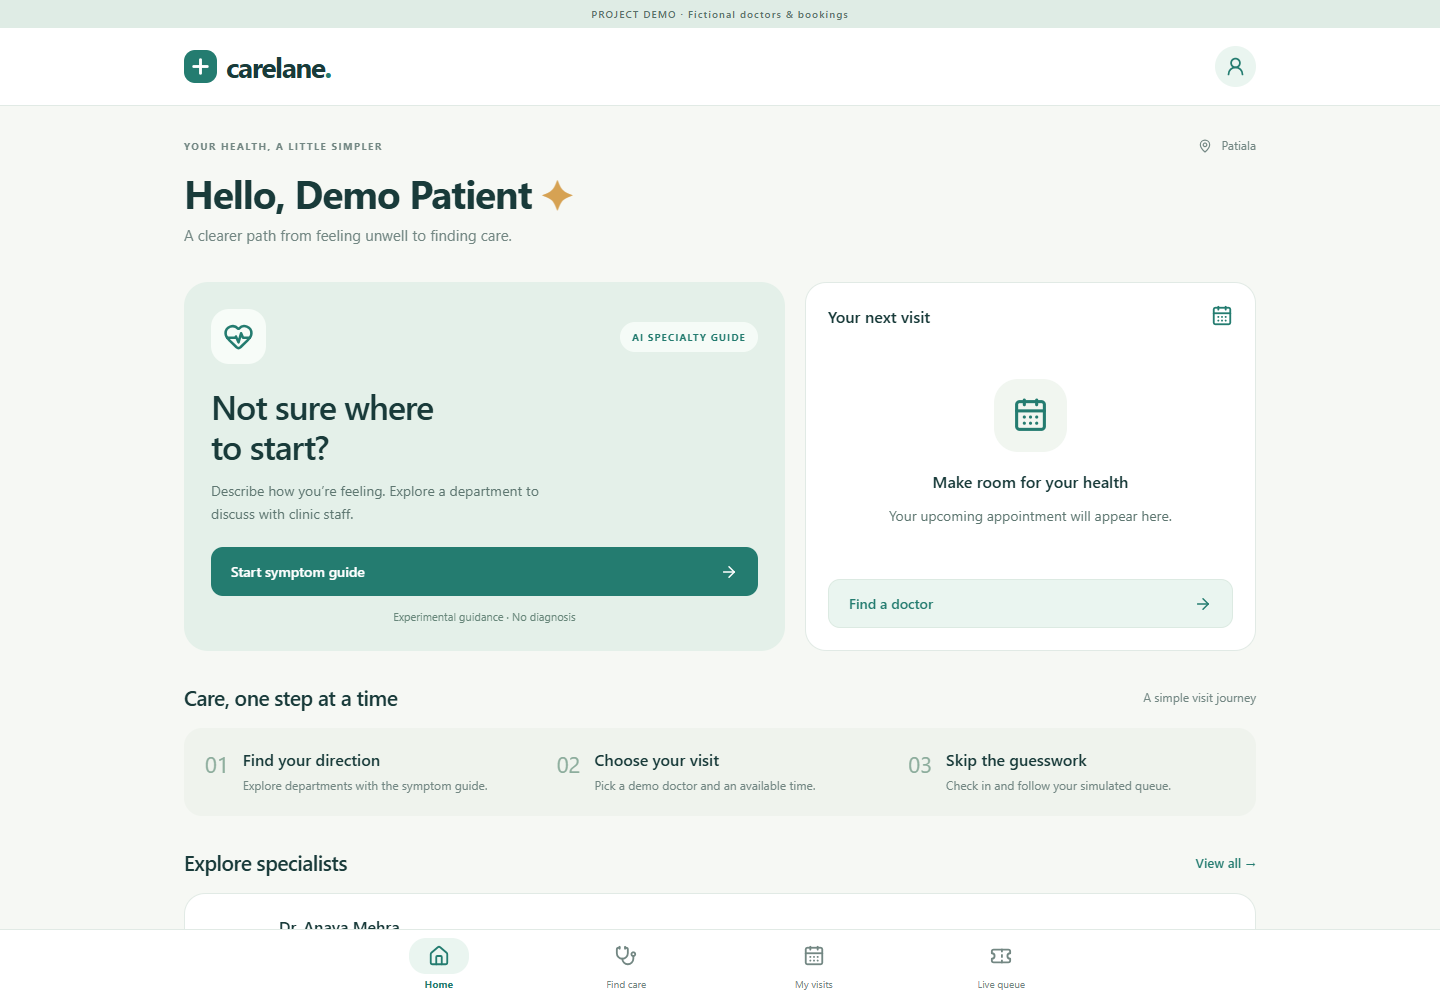
\includegraphics[width=\textwidth]{home-desktop.png}
\caption{Patient home screen captured during the 9 September verification. Doctors and bookings in this version are fictional.}
\end{figure}

\subsubsection{Queue workflow and service interface}
The demo appointment transitions from \texttt{booked} to \texttt{checked\_in}, then \texttt{ready} and finally \texttt{completed}. A pre-check-in appointment may instead become \texttt{cancelled}. Check-in starts a demonstration with three fictional patients ahead. The demo desk advances that count explicitly rather than implying an active clinic feed.

CatBoost estimates are used for General Medicine, Dermatology and Orthopedics, the departments represented in queue training. Other fictional departments use a simple arithmetic waiting estimate. Both approaches are displayed as simulated estimates. Immediate check-in for a future appointment is intentionally permitted for the demonstration and is not a proposed real-clinic scheduling rule.

\begin{table}[H]\centering\small
\begin{tabularx}{\textwidth}{p{0.43\textwidth}Y}\toprule Service operation & Purpose \\ \midrule
Create session & Obtain an anonymous demo token. \\
List providers and slots & Browse fictional doctors and available candidate times. \\
Request guidance & Run the local specialty model on an example description. \\
Create/list appointments & Save a booking or retrieve the current session's visits. \\
Cancel/check in & Perform permitted visit-state transitions. \\
Read queue/demo advance & Refresh simulated status or explicitly move the demo queue. \\
\bottomrule\end{tabularx}
\caption{Implemented patient-service operations.}
\end{table}

\begin{figure}[H]\centering
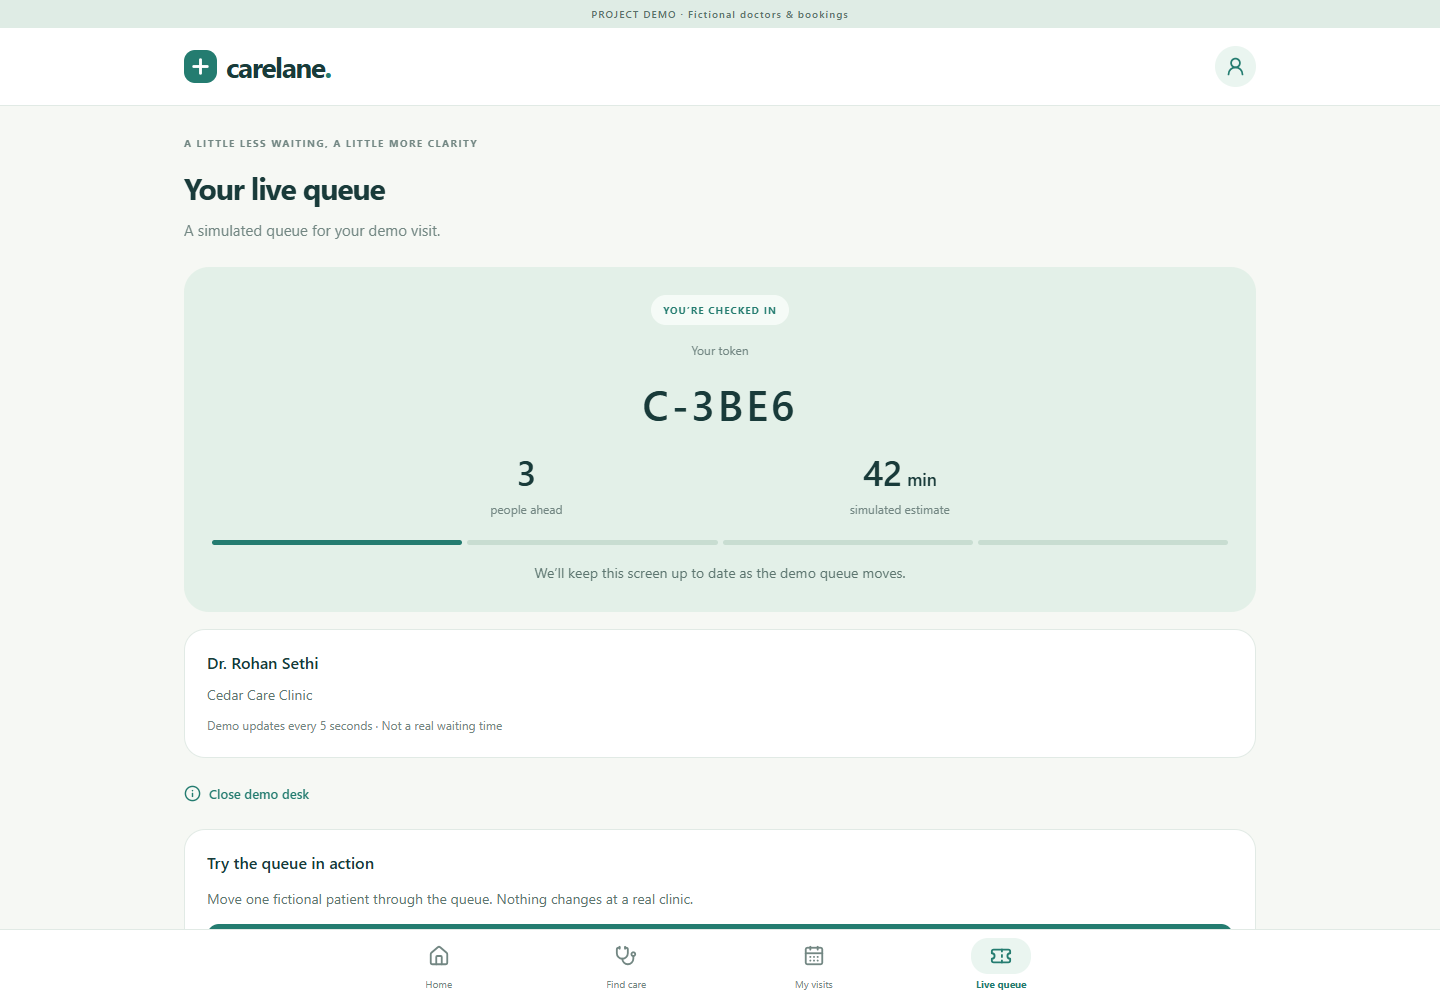
\includegraphics[width=\textwidth]{queue.png}
\caption{Recorded queue screen. The displayed waiting time is an example simulation output, not measured hospital availability.}
\end{figure}

\subsubsection{Experiment dashboard and reproducibility}
The local research dashboard presents saved classification metrics, training curves, confusion matrices, queue results and logs. CSV prediction exports, model metadata and a research bundle support later analysis. The training journal records run starts, epoch summaries, completion events and model locations. Environment records, download checksums and source hashes help connect reported values to the original experiment.

The project also provides a double-click application launcher and written reproduction instructions. The research report server and patient application use separate local endpoints, keeping analysis artifacts independent from demo appointment state.

\chapter{Results and Evaluation}
\section{Testing Methodology}
Text model hyperparameters and transformer checkpoints are selected on validation macro-F1. Test results below come from 212 retained descriptions. Accuracy measures the fraction of correct first-ranked labels, while macro-F1 averages the class-wise F1 scores and gives equal weight to each class:
\begin{align}
\mathrm{Accuracy} &= \frac{\text{correct predictions}}{N},\\
F_{1,k} &= \frac{2P_kR_k}{P_k+R_k},\qquad
\mathrm{MacroF1}=\frac{1}{K}\sum_{k=1}^{K}F_{1,k}.
\end{align}
Top-three accuracy reports whether the reference label appears among the first three ranked outputs. It does not establish that any suggested department is appropriate for a real patient.

Queue evaluation uses mean absolute error (MAE) and root mean squared error (RMSE), expressed in minutes:
\begin{align}
\mathrm{MAE}&=\frac{1}{N}\sum_{i=1}^{N}|y_i-\hat y_i|,\\
\mathrm{RMSE}&=\sqrt{\frac{1}{N}\sum_{i=1}^{N}(y_i-\hat y_i)^2}.
\end{align}
Results are compared with the simulator experiment's simple waiting-time baseline. They quantify error within the generated data, not clinical effectiveness.

Software verification combines backend tests, a real browser journey, static type checking and export builds. It is separate from model evaluation: an application can correctly carry a prediction through a workflow while the model itself remains clinically unvalidated.

\section{Performance Metrics}
\subsection{Text Classification Results}
\begin{table}[H]\centering\small
\begin{tabularx}{\textwidth}{Yrrr}\toprule Model and target & Val. macro-F1 & Test accuracy & Test macro-F1 \\ \midrule
TF-IDF + LR: condition & 0.9516 & 94.34\% & 0.9430 \\
TF-IDF + LR: specialty & 0.9674 & 96.70\% & 0.9683 \\
DistilBERT: specialty & 0.9768 & 95.75\% & 0.9596 \\
\bottomrule\end{tabularx}
\caption{Latest saved classification results. All models use 673 training, 168 validation and 212 test records; specialty labels are unreviewed proxies.}
\end{table}

The condition baseline correctly classifies 200 of 212 test descriptions. The specialty baseline correctly classifies 205, compared with 203 for DistilBERT. The specialty baseline therefore has a 0.94 percentage-point test accuracy advantage in this experiment, while DistilBERT has the higher validation macro-F1. These small differences are descriptive; no statistical significance study or multi-seed comparison has been performed.

Top-three accuracy is 99.53\% for condition classification and 100\% for both specialty classifiers on this small test partition. The latter score must be interpreted alongside the nine-label proxy task, dataset size and lack of clinical annotation.

\begin{figure}[H]\centering
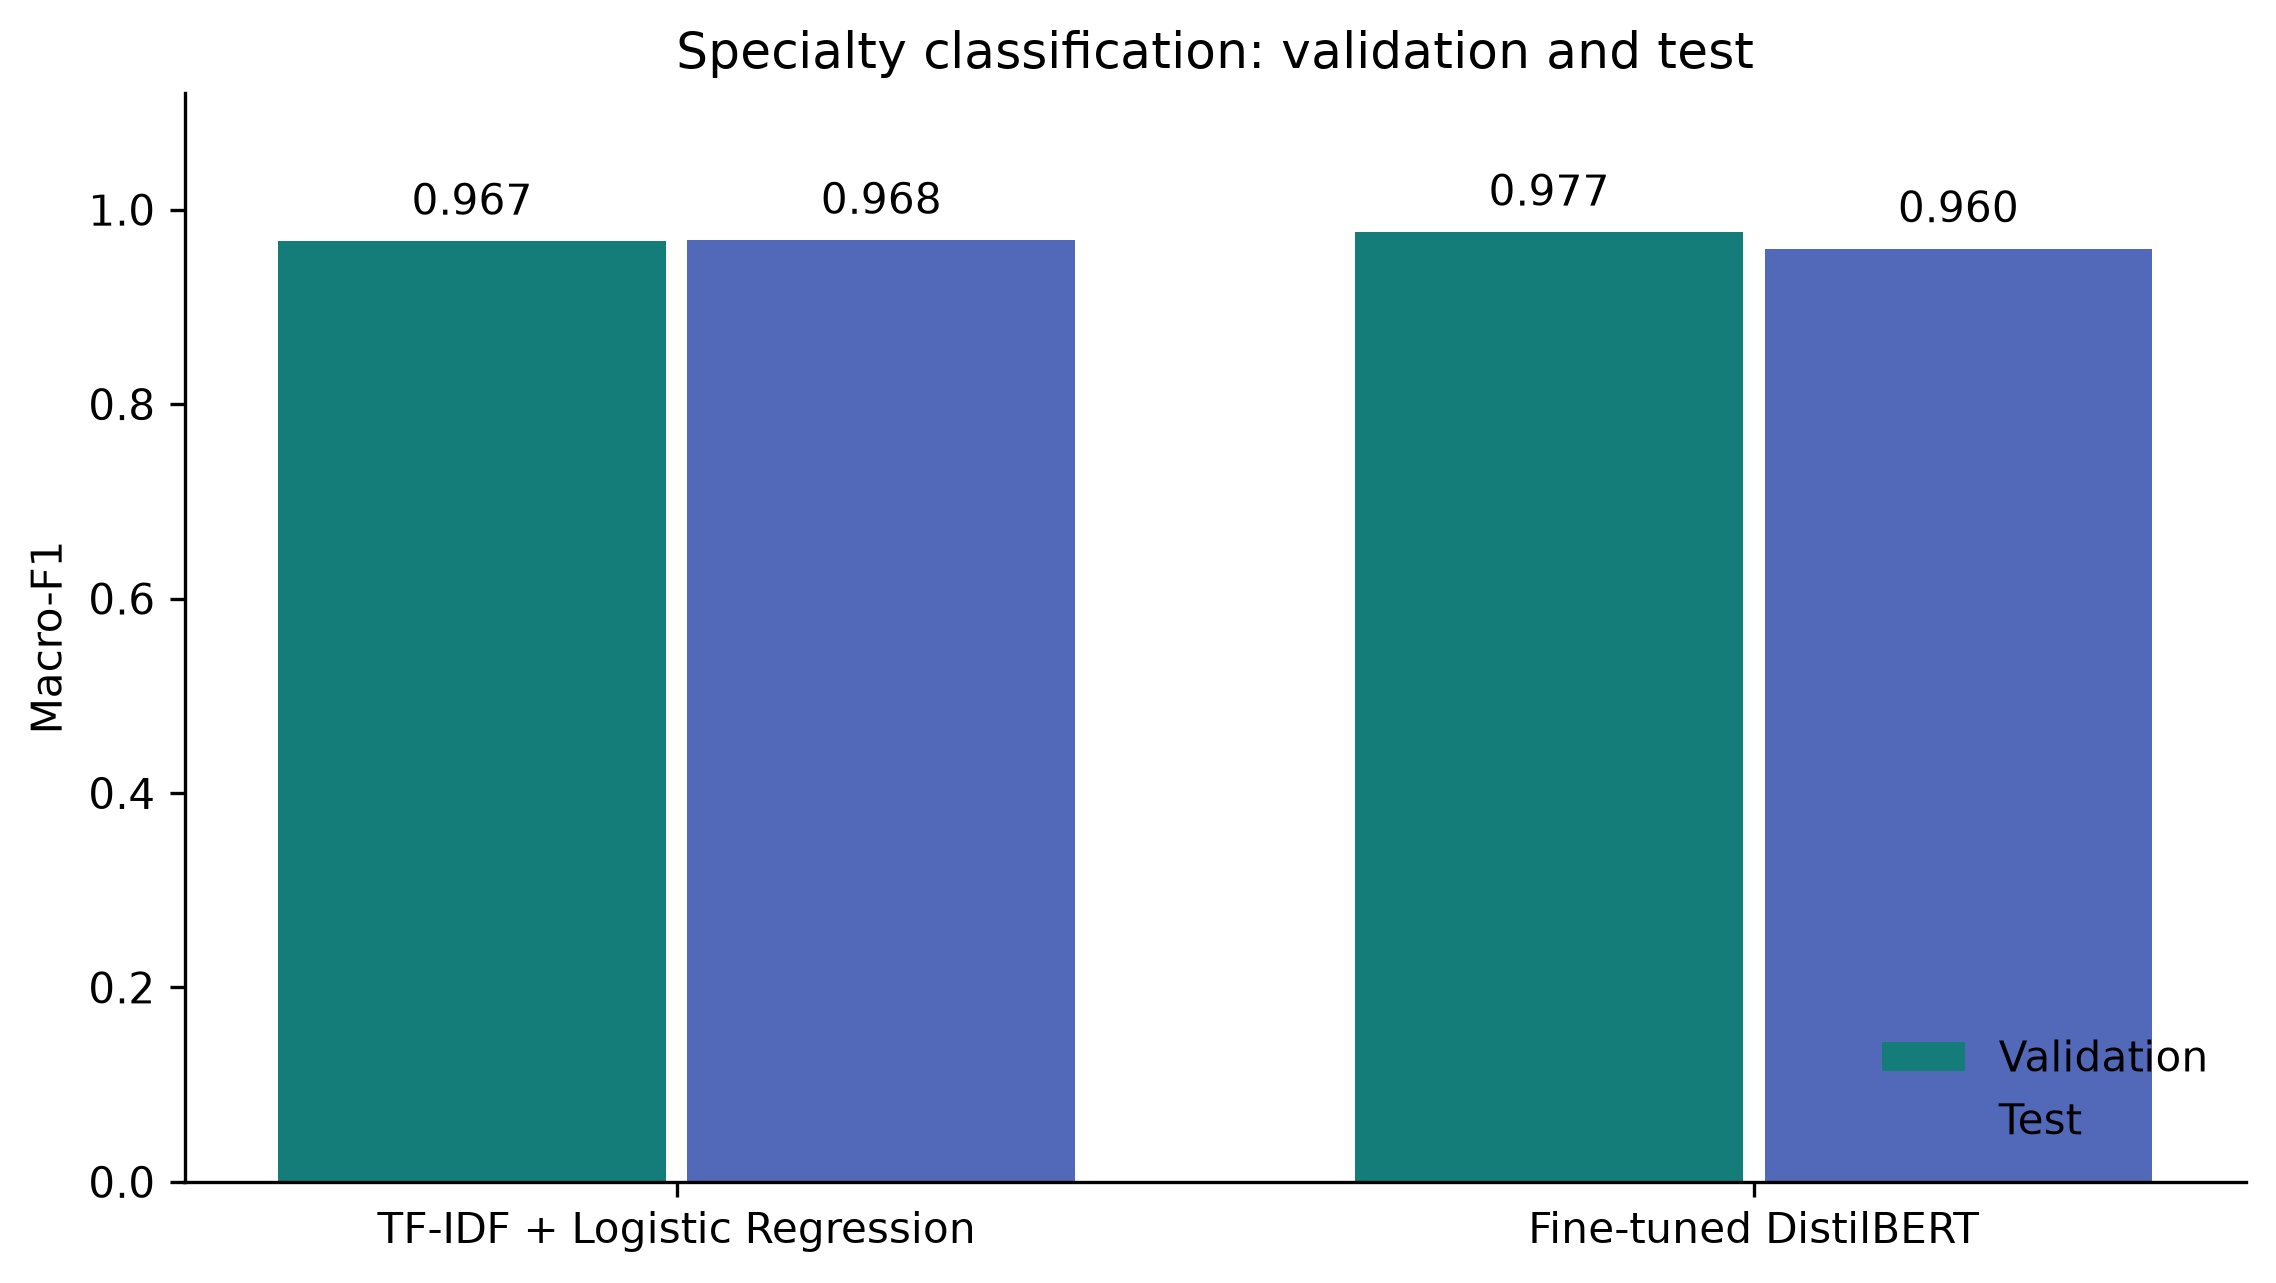
\includegraphics[width=\textwidth]{01_specialty_comparison.png}
\caption{Saved comparison figure for the two specialty models. Numerical conclusions in this report are taken from metric JSON and prediction exports.}
\end{figure}

\subsection{Training History and Recorded Duration}
The eight-epoch DistilBERT run selected epoch eight, with validation accuracy 98.21\% and macro-F1 0.9768. Training loss at that epoch was approximately 0.0253. These are training/validation observations; the separate test accuracy is 95.75\%.

\begin{table}[H]\centering
\begin{tabular}{lr}\toprule Recorded run & Duration (seconds) \\ \midrule
Condition TF-IDF + Logistic Regression & 5.97 \\
Specialty TF-IDF + Logistic Regression & 2.81 \\
Specialty DistilBERT, eight epochs & 94.79 \\
Queue CatBoost & 18.91 \\
\bottomrule\end{tabular}
\caption{Script-reported run durations. They exclude installation and downloads and are not controlled inference-latency or hardware benchmarks.}
\end{table}

The baseline durations include comparison of three regularization values. The transformer duration covers the measured fine-tuning, selection/evaluation and saving sequence, whereas the queue run uses a different dataset and objective. Comparing these durations is useful for understanding local development effort, but not for claiming a general speed advantage under standardized conditions.

\begin{figure}[H]\centering
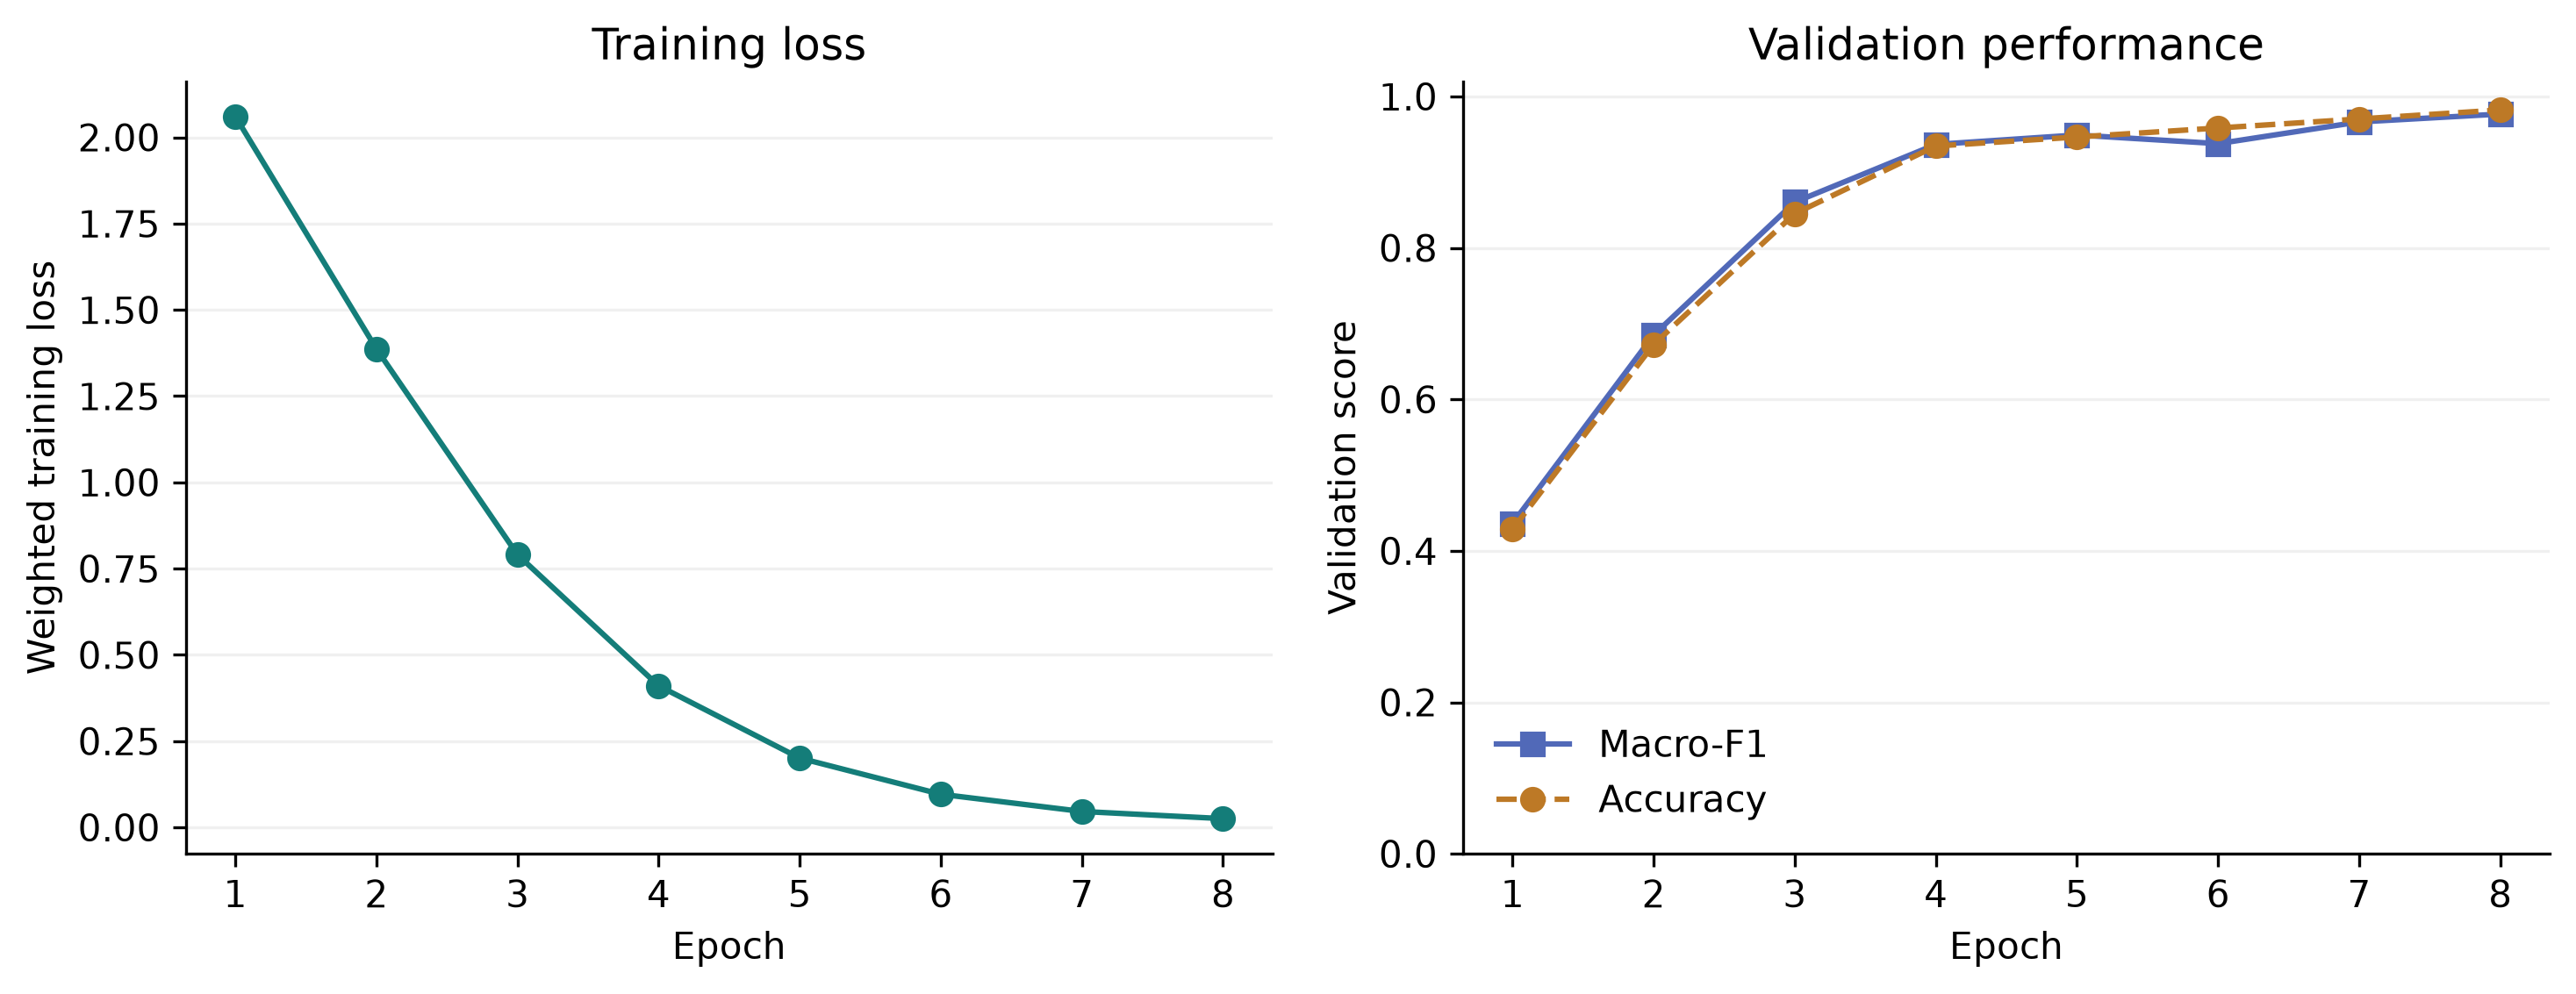
\includegraphics[width=\textwidth]{02_distilbert_training_curves.png}
\caption{Saved eight-epoch DistilBERT training and validation curves. Checkpoint selection used validation macro-F1.}
\end{figure}

\subsection{Queue Estimation Results}
\begin{table}[H]\centering
\begin{tabular}{lrr}\toprule Measure & Validation & Test \\ \midrule
CatBoost MAE (minutes) & 4.795 & 5.464 \\
Simple baseline MAE (minutes) & 5.636 & 6.378 \\
CatBoost RMSE (minutes) & -- & 8.908 \\
\bottomrule\end{tabular}
\caption{Queue results on simulated later-day partitions. Validation RMSE is not reported in the saved metric summary.}
\end{table}

The reduction in test MAE is approximately 0.914 minutes, or 14.34\% relative to the simple baseline. This is a reduction in prediction error on simulated data, not a 14.34\% reduction in real patient waiting time. Patients ahead has the largest reported feature importance (55.47\%), followed by active doctors (22.50\%). These model importance values describe the fitted simulator experiment and are not causal estimates.

\begin{figure}[H]\centering
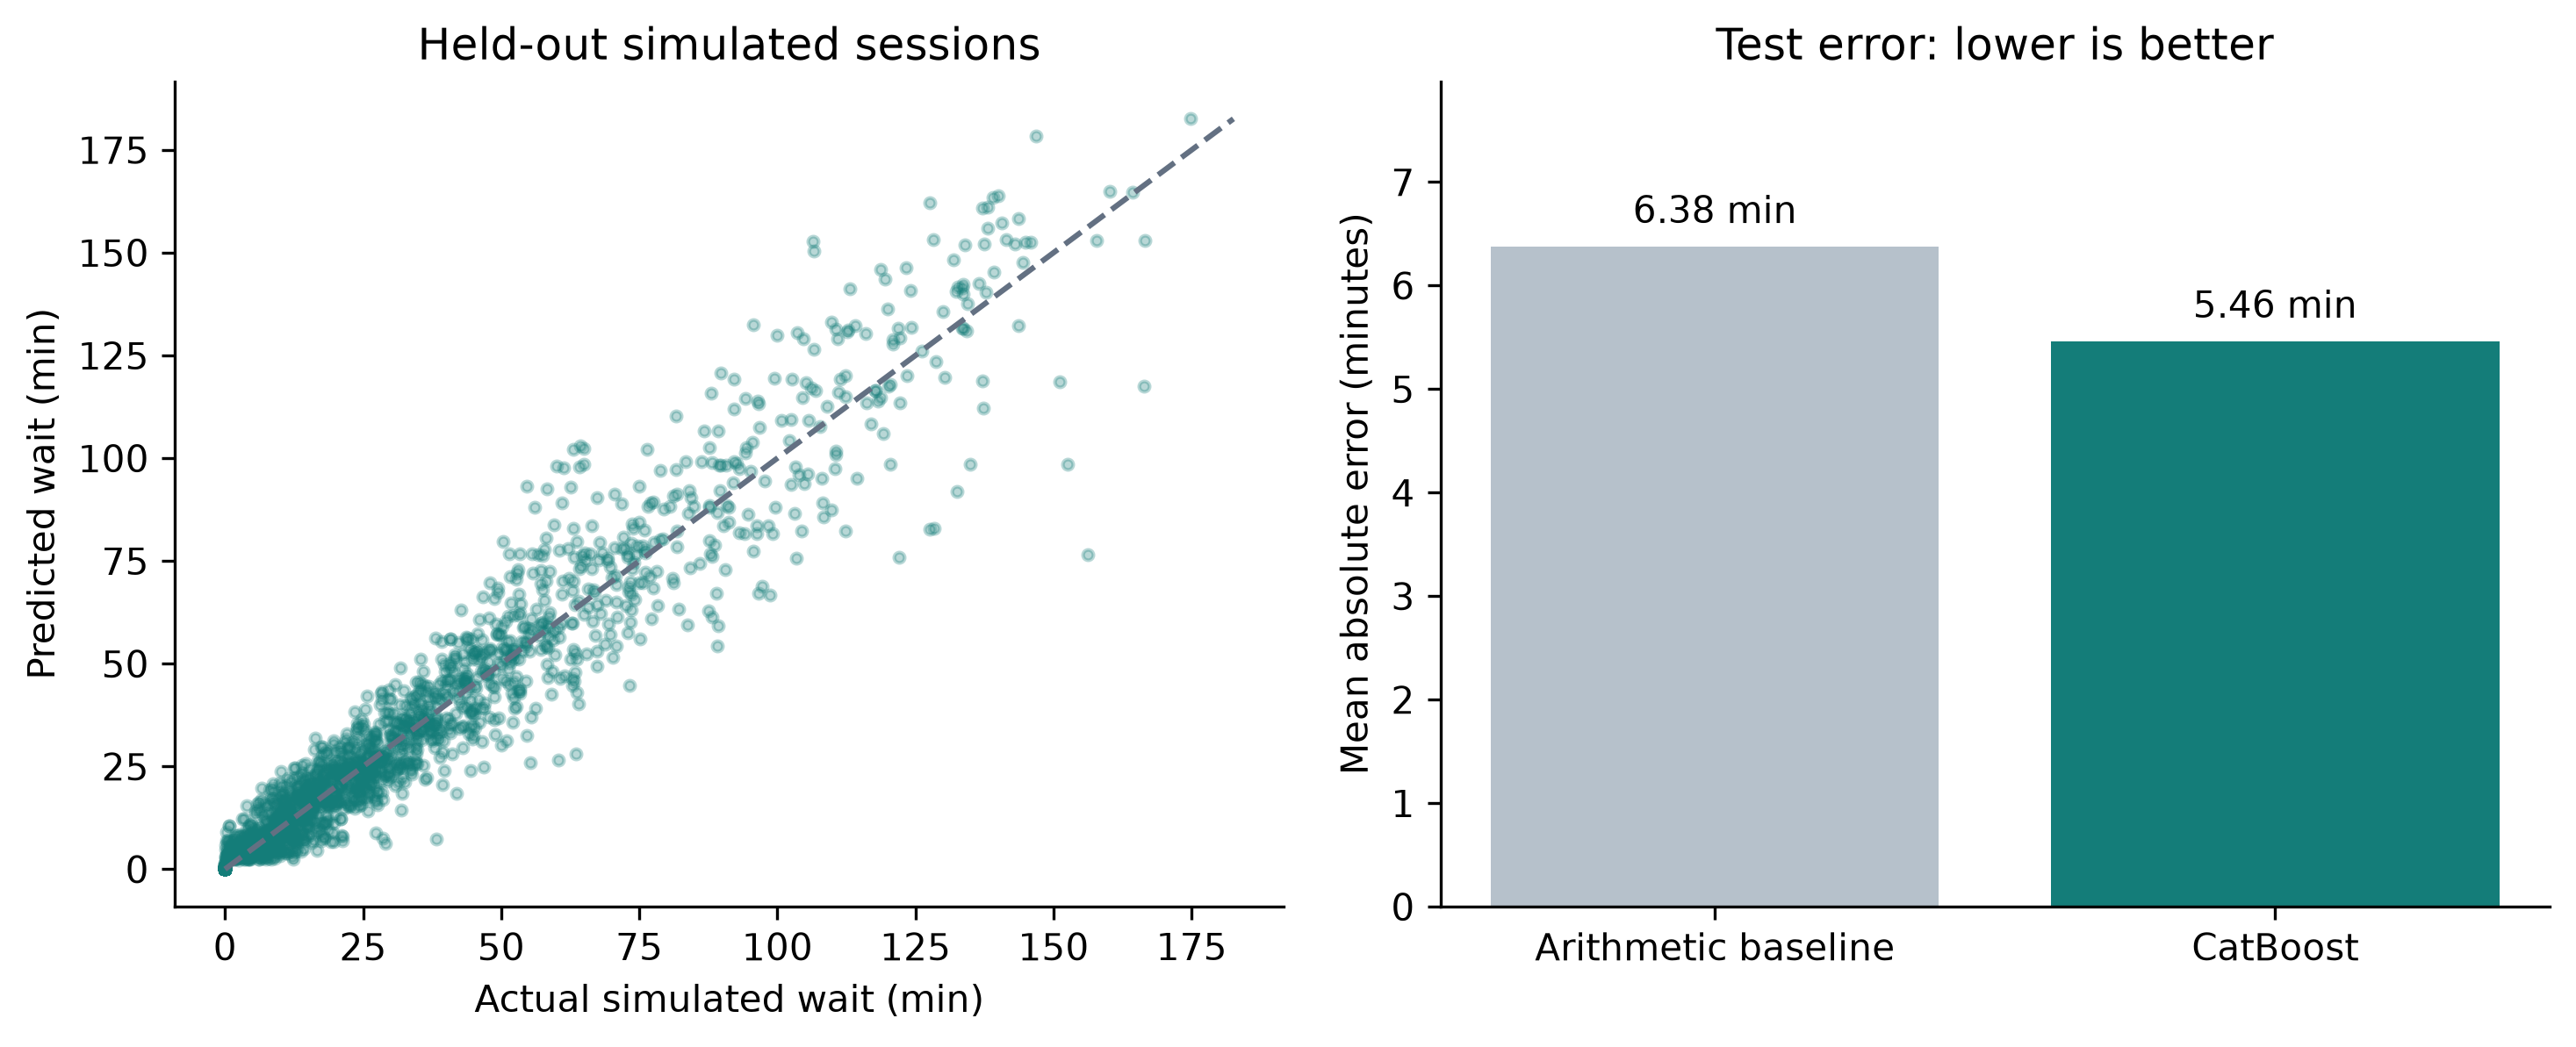
\includegraphics[width=\textwidth]{04_queue_simulation_results.png}
\caption{Saved queue simulation evaluation figure. No prospective hospital observations were used.}
\end{figure}

\subsection{Application Verification}
The saved 9 September validation record reports four passing backend tests in 8.79 seconds, with two upstream deprecation warnings. Covered behaviours include session ownership, unauthorized access, repeated booking requests, concurrent slot contention, cancellation releasing a slot, queue progression, invalid inputs and real local-model inference.

The final browser record contains nine successful checks: home loading; a saved-model Dermatology suggestion for the example input; doctor filtering and slots; booking persistence after reload; check-in; queue progression from three people ahead through completion; a 390-by-844 viewport without horizontal page overflow; search with no matching results; and an unavailable-service error. No uncaught browser errors were recorded in that run.

TypeScript checking, a web export and an Android JavaScript/Hermes export also passed. These build checks do not demonstrate installation, native permissions or behaviour on a physical Android device. The signed application package remains future work.

\section{Analysis}
\subsection{What the Evidence Supports}
The results demonstrate a functioning data-to-model pipeline and a connected local application workflow. A relatively compact word/character baseline is competitive with the transformer on the retained text data. Using the specialty baseline in the current patient service is consistent with the observed test result and its simple local deployment. DistilBERT remains a useful comparison model rather than being described as automatically superior because it is more complex.

The queue experiment shows that CatBoost can learn useful relationships in the simulator beyond the simple baseline. The software tests show persistence and state-management correctness for a bounded demonstration. Together, these findings support an engineering proof of concept.

\subsection{Limitations and Threats to Validity}
\begin{itemize}
\item \textbf{Dataset scope:} the text corpus is small, English-only and publisher-described as LLM-rewritten. It may differ substantially from real patient descriptions.
\item \textbf{Label validity:} specialty targets are condition-derived, unreviewed proxy labels. They cannot establish professional routing agreement.
\item \textbf{Leakage and reuse:} exact-name removal and similarity grouping reduce some shortcuts but cannot exclude semantic overlap. Test data have been seen in multiple development runs.
\item \textbf{Statistical evidence:} no independent external test set, multiple-seed study, confidence intervals, subgroup analysis or significance testing has been completed.
\item \textbf{Calibration:} classifier outputs are uncalibrated scores, not probabilities of disease or clinical correctness.
\item \textbf{Simulation scope:} the FCFS simulator excludes important real-world effects such as priority handling, emergencies, breaks and cancellations in queue generation.
\item \textbf{Deployment scope:} fictional providers, local anonymous sessions and synthetic queue controls are not production hospital integrations. No clinical safety or production security assurance is claimed.
\end{itemize}

\chapter{Conclusion}
\section{Summary of Work}
The project has progressed from a combined healthcare-assistance concept to a local, testable prototype. Completed work includes dataset acquisition and audit, condition and specialty baselines, an eight-epoch DistilBERT fine-tuning run, simulated queue modelling, saved experiment reporting, and a patient interface backed by persistent demo appointment state. The app demonstrates a complete symptom-guidance-to-queue journey using the saved specialty baseline.

The available artifacts include trained model files, evaluation JSON, row-level predictions, download manifests, environment records, source hashes, a training journal, research figures, screenshots and test records. These make the reported work inspectable and reproducible within the recorded environment.

\section{Key Findings}
The strongest first-ranked specialty test accuracy among the saved models is 96.70\% for TF-IDF plus Logistic Regression, while DistilBERT reaches 95.75\% and has higher validation macro-F1. CatBoost achieves test MAE of 5.464 minutes against 6.378 minutes for the simple simulation baseline. The tested patient application preserves bookings across reloads and supports the expected queue transitions.

These findings should be read as prototype and experimental results. They do not prove diagnostic correctness, clinically appropriate routing, reduced hospital waiting time or readiness for patient use.

\section{Future Work and Recommendations}
\begin{enumerate}
\item Complete the public-care directory after a location is confirmed, verify doctor/hospital/clinic details against official sources, and integrate the draft redesigned screens. Keep real contact information distinct from demo booking actions.
\item Collect or obtain suitable clinician-reviewed, consented data and evaluate on an independent external set. Review specialty definitions before extending the routing task.
\item Conduct multiple-seed comparisons, error analysis and probability calibration where appropriate. Report uncertainty rather than optimizing repeatedly against the same test set.
\item Replace simulated queue assumptions with appropriately governed operational data; account for priority, interruptions, cancellations and changing staffing.
\item Add production authentication, access control, data retention and audit policies, followed by security assessment.
\item Verify the application on physical Android devices and produce a signed build. Test networking, permissions, failure recovery and accessibility.
\item Integrate a real appointment system only with provider authorization and confirmed availability. Add notifications and staff controls after the underlying workflow is validated.
\end{enumerate}

\section{Final Remarks}
Carelane currently provides a foundation for demonstrating machine-learning integration within a healthcare-themed software system. Its main contribution at this stage is the connection between reproducible experiments and a working patient workflow, with clear separation between research outputs and real healthcare actions. The next development phase should prioritize verified data, robust integration and evaluation rather than treating prototype accuracy as evidence of clinical readiness.

\appendix
\chapter{Reproducibility and Evidence}
\section{Artifact Locations}
Paths below are relative to the \texttt{healthcare-ai} project directory.
\begin{table}[H]\centering\small
\begin{tabularx}{\textwidth}{p{0.43\textwidth}Y}\toprule Location & Evidence \\ \midrule
\texttt{reports/data\_audit.json} & Duplicates, similarity threshold and retained partitions. \\
\texttt{reports/*\_metrics.json} & Model settings, validation/test metrics and environment. \\
\texttt{reports/*\_predictions.csv} & Row-level saved predictions. \\
\texttt{TRAINING\_JOURNAL.txt} & Run and epoch events. \\
\texttt{reports/download\_provenance.json} & Revisions and checksums for downloaded assets. \\
\texttt{reports/research\_assets/} & Figures, captions, tables and source snapshots. \\
\texttt{reports/app/} & Screenshots, browser result JSON and validation record. \\
\texttt{healthcare\_ml/} & Preparation, training, inference and service source. \\
\texttt{patient-app/} & Expo application source and browser checks. \\
\bottomrule\end{tabularx}
\caption{Evidence supporting this report.}
\end{table}

\section{Reproduction Procedure}
Use the saved environment and dataset/model revisions. Data preparation should precede model training, and hyperparameters should be selected using validation data. The transformer training entry point supports an epoch argument; the reported run used eight epochs. A new training run may overwrite the latest metrics and artifacts, so archive the existing results before attempting a new experiment.

For application demonstration, the supplied \texttt{START\_APP.bat} launcher starts the patient service and Expo browser preview. The project instructions document local ports, model paths and optional phone testing. Run the saved backend and browser checks when changing the workflow. Rebuilding an Android JavaScript bundle is not equivalent to installing and testing a signed APK.

\section{Team and Reporting Notes}
The team members are Pranshu Sharma, Shashwat Mishra and Mayank Kalra; the latter two surnames and the UCS503P/third-year COE programme information were checked against the supplied project-proposal PDFs. Individual contribution assignments have not been supplied and are therefore not invented here. The earlier two-person allocation file was a plan and should not be used as evidence of completed contributions by this three-person team. Initial code, experiments and report preparation were AI-assisted; the team should review and understand the implementation and comply with its course's disclosure requirements.

The cover retains the institution and mid-semester evaluation label from the supplied TIET template. Roll numbers, group number and faculty name are marked for completion. The document describes current progress, including explicit unfinished work; it does not claim all originally proposed capabilities are delivered.

\begin{thebibliography}{99}
\addcontentsline{toc}{chapter}{Bibliography}
\bibitem{gretel} Gretel AI. \emph{symptom\_to\_diagnosis dataset and dataset card}. Hugging Face. Recorded revision: \texttt{722cfb0e11f8ae37339c7f573b5e10429b94df49}. Download recorded 6 September 2026. \url{https://huggingface.co/datasets/gretelai/symptom_to_diagnosis}.
\bibitem{distilbert} Hugging Face. \emph{distilbert-base-uncased model card and checkpoint}. Recorded revision: \texttt{12040accade4e8a0f71eabdb258fecc2e7e948be}. Download recorded 6 September 2026. \url{https://huggingface.co/distilbert/distilbert-base-uncased}.
\bibitem{sklearn} scikit-learn developers. \emph{Text feature extraction and Logistic Regression documentation}. Implementation used in the project: scikit-learn 1.9.0. \url{https://scikit-learn.org/stable/modules/feature_extraction.html}.
\bibitem{catboost} CatBoost developers. \emph{CatBoostRegressor documentation}. Implementation used in the project: CatBoost 1.2.10. \url{https://catboost.ai/docs/en/concepts/python-reference_catboostregressor}.
\bibitem{expo} Expo. \emph{Expo SDK 57 reference}. \url{https://docs.expo.dev/versions/v57.0.0/}.
\bibitem{internal} Carelane project. \emph{Saved training metrics, data audit, training journal and application validation artifacts}, 6--9 September 2026. Local project evidence summarized in Appendix A.
\bibitem{template} \emph{TIET-Report-Template}, supplied Overleaf project; \texttt{tietreport.cls} v1.0.4, 3 September 2026. \url{https://www.overleaf.com/read/rjgcdqyqkxnd}.
\end{thebibliography}
\end{document}
